\chapter[ GPGPU-Based Implementation of a finite difference algorithm]{GPGPU-Based Implementation of \\ a finite difference algorithm}


The objective of this chapter is to give an overview of the basic implemenation of an algorithm using finite difference schemes.
The source code used for the computations is based on an existing and validated version from A. Tilgner.
It was furthermore extended by the immersed boundary methods, which will be explained in more detail in chapter \ref{CHAPTER:IBM}.
Especially in this context we will introduce some aspects of GPGPU\footnote{General Purpose Computation on Graphics Processing Uni}-Computing
with the CUDA \footnote{Computing Uniform Device Architecture} architecture.
For the computations the  in this thesis Tesla C1060 and Tesla K20m GPUs by NVIDIA were used.%, the complete system configurations can be looked up at (AX.X).

In this chapter, all informations related to GPGPU-Computing and CUDA are adapted from the CUDA Programming Guide and the CUDA Best Practices Guide from NVIDIA
\citep{CUDAPG}, \citep{CUDABP}. (Algorithm pc tilner and testing)

\section{GPGPU-Computing with CUDA}

CUDA is an architecture developed by NVIDIA to enable an easy approach to the Implementation of GPGPU-based algorithms.
The underlying idea is to hide the complexity of the hardware under a more high oriented and generalized software abstraction layer.
This is done by introducing some additional programming language extensions i.e. in C/C++\footnote{WIR BENUTZEN C/C++ /PYTHON ETC},
furthermore it is necessary to use a CUDA suited compiler like NVCC.

\subsection{Hardware and Memory Architecture}

A cuda device contains an array of so called streaming multiprocessors (SM).
Each of these SMs contains a group of small execution units, which are called cuda cores.
For the exchange of data between different SMs, cuda cores and the CPU side of the computer, there exists different
types of memory, as shown  in figure (X).
\newpage

\begin{figure}[!tbp]
      \centering
        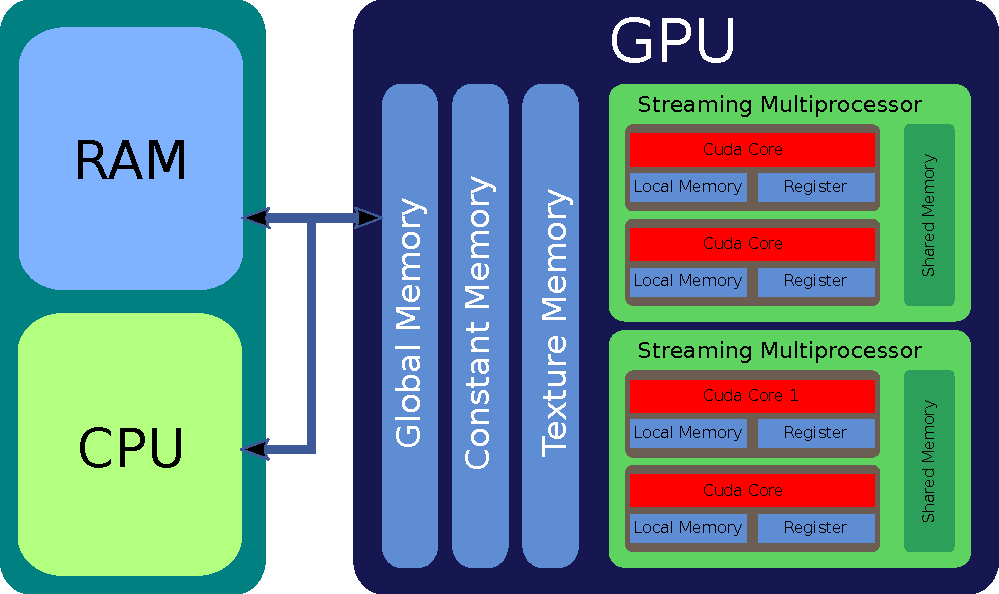
\includegraphics[width=0.9\textwidth]{gfx/cuda/gpu.pdf}
          \caption{Memory layout of a Nvidia-GPU}
    \label{fig:gpu_grid}
\end{figure}

\begin{description}
    \item[Global Memory] The global memory is the largest memory on the gpu and can be accessed by all cuda cores.
                         It is  used to exchange data with the RAM and distribute it between different SMs.
                         Writing and reading from the global memory is slow. A part of global memory can furthermore be used a constant memory, in this case
                         multiple memory accesses on the same location are temporary cached.
                         In addition the use of the global memory as a texture memory is possible. The memory access is then spatially cached.


    \item[Shared Memory] Each SM contains a shared memory, much smaller than the global memory \footnote{Around 16kb on c1060 and 64kb on k20m}. It is accessible
                         by all cuda cores of the SM.
                         This memory type is much faster (x100) than the global memory and is usefull when multiple operations
                         by different cuda cores are carried out on the same data.

    \item[Register / Local Memory] Each cuda core posseses an own set of registers and local memory.
                                   The register access is slightly faster than the access  on the shared memory.
                                   Local memory access is very slow since
                                   it is created on the global memory, when the cuda core runs out of resources.
\end{description}

\clearpage

\subsection{Thread Management}

In order to distribute the workload between different SMs and cuda cores an additional syntax is necessary.
The CUDA API therefore  introcuces the notion of a thread and a block.

\begin{description}
    \item[Thread] A Thread is the software abstraction of a single cuda core. It can be identified with
                   a maximum of three IDs, \textbf{threadIdx.x}, \textbf{threadIdx.y} and\textbf{threadIdx.z}.

    \item[Block] A block is defined as a group of threads, i.e. in Fig. \ref{cuda:grid_example} a Block contains of 64 threads.
                 There  is no direct hardware equivalent to a block.
                 A block is identified by a maximum of two IDs, \textbf{blockIdx.x} and \textbf{blockIdx.y}

    \item[Blocksize] The blocksize is defined at the beginning of a cuda programm. It determines how
                    many threads run inside a block. In Fig. \ref{cuda:grid_example} the blocksize is set to (8, 8).
                    each thread has a threadIdx.x and threadIdx.y.

    \item[Gridsize] The gridsize defines the total number of blocks, i.e. (2, 2) in the example.
\end{description}

These abstractions are necessary to enable a high workload on the gpu.
For the distribution of data the grid of blocks is used, each block can be dynamically assigned to a different SM.

\begin{figure}[!bp]
      \centering
        \resizebox{0.5 \textwidth}{!}{
       \import{gfx/cuda//}{grid.pdf_tex}
        }
       \caption{Segmentation of the $y, z$ plane of the simulation domain into a grid of Blocks.
                 Eeach block contains a grid with 8x8 threads.}
       \label{cuda:grid_example}
\end{figure}

\subsection{Performance Considerations}

As a conlusion the algorithm should fulfill the following prerequisites.
The global memory should be used for data transfer and distribution, with as little as possible global reads.
Immediatly after the data is transfered to the shared memory there should be as many as possible computations before transfering
it back. Furthermore all memory accesses should be optimized, see chapter (X.X).

\subsection{Pre Processing}

\label{cuda:prepro}
Before integrating the equations of motion we need to define the initial state of our system, as stated in section (X)
This includes the flow variables but also a set of parameters.
For one flow variable we need three different memory allocations.
The first allocation will be one the system RAM.
-hdf5 python
The second and third allocation reside on the global memory of the gpu.
This is due to the fact that the runge kutta method uses two storage registers, during the timestep execution.
The fields for all variables are summarized in table (1).

\begin{center}
    \begin{tabular}{ | l | l | l | l |}
    \hline
    Variable & Field on RAM & GPU Field & 2nd GPU Field \\
    \hline
    Velocity in x-direction $v_x$  & \texttt{vx}   &  \texttt{vx\_d}   & \texttt{vx2\_d}   \\
    Velocity in y-direction $v_y$  & \texttt{vy}   &  \texttt{vy\_d}   & \texttt{vy2\_d}   \\
    Velocity in z-direction $v_z$  & \texttt{vz}   &  \texttt{vz\_d}   & \texttt{vz2\_d}   \\
    Density  $\rho$  & \texttt{rho}  &  \texttt{rho\_d}  & \texttt{rho2\_d}  \\
    \hline
    \end{tabular}
\end{center}
The parameter set defines different attributes of the system.
This can be physical attributes like the rayleigh- or prandtl-number, numerical parameters like the grid resolution
memory layout

\clearpage

\section{Time Step Algorithm}

In this section an overview of the computation of a single time step will be given.
The simulation domain for this example is a cube of length $l$ and the resolution $N$ in three dimensions.
It is presumed that all variables are allocated on the global memory of the gpu, see Sec. \ref{cuda:prepro}.

The simulation domain is then divided into a grid of  $N/8 \times N/8$ blocks, like in Fig. \ref{cuda:grid_example}.
Each block contains a total number of 8x8x4 threads.
The threadIdx.z defines which variable will be used for the computation, i.e. threadIdx.z=0 corresponds to $\rho$, threadIdx.z=1 to $v_x$.










\clearpage

During execution time each cuda core is executed as a thread, in an SIMD\footnote{Single Instruction Multiple Device}-like behaviour.
This means every cuda core on one SM executes the same instruction set simultaneously. To differentiate between different cuda cores,
each get assigned to a different \textbf{ThreadId}.
With the declaration of a block dimension, we define how many threads are executed in parallel.
The block dimension can be up to 3-dimensions. In this case each cuda core will be assigned to a ThreadId in x, y and z direction.
A collection of threads with this grid structure is called a block.
Since the

The grid dimension describes the
NEUSCHREIBEN

%\begin{figure}[!tbp]
%  \centering
%  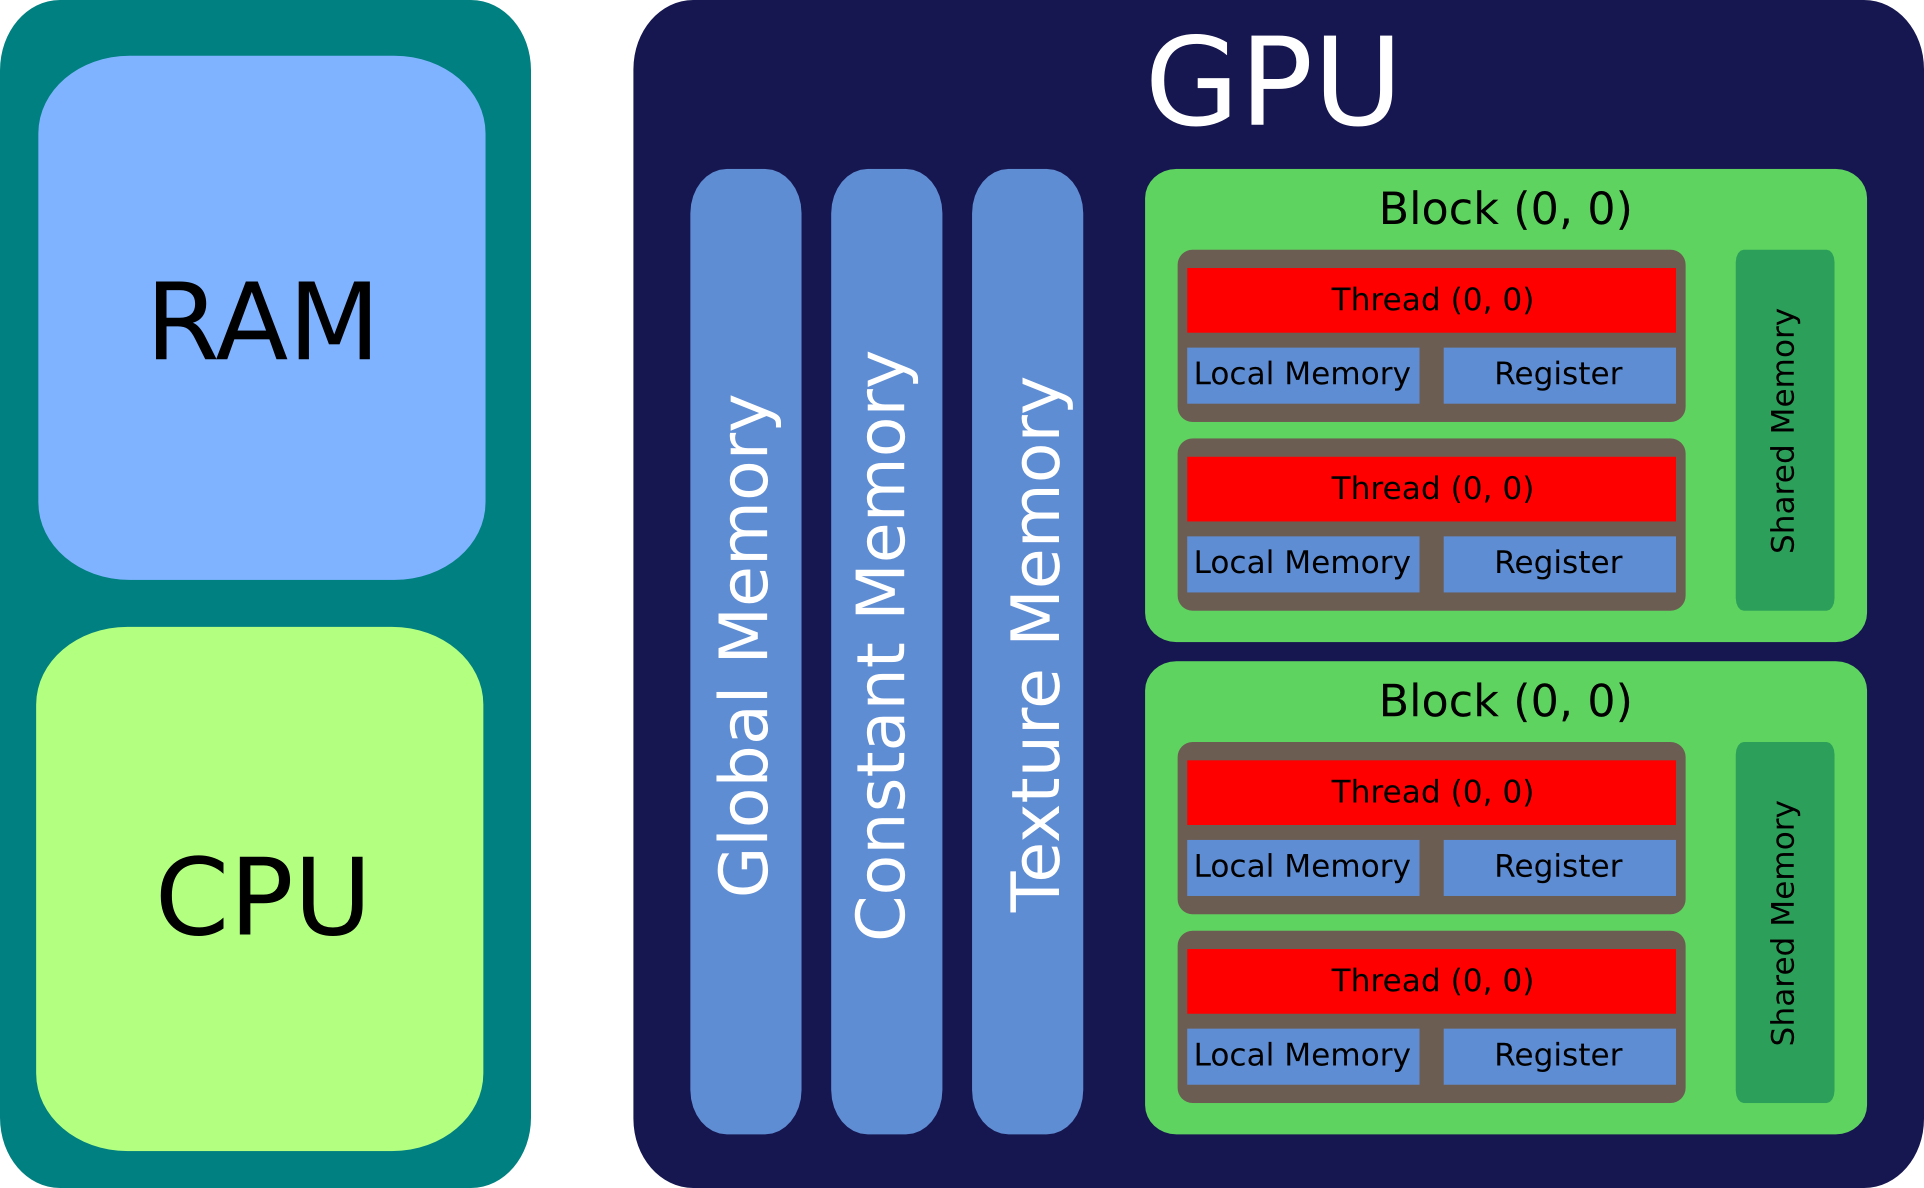
\includegraphics[width=0.8\textwidth]{gfx/cuda/gpu.png}\label{fig:gpu_grid}
%  \caption{Block and grid layout for a two dimensional array.}
%\end{figure}

To illustrate the usage of grid and block dimensions, let us consider a two-dimensional array of shape 16x16, as shown in figure ().
-copy to gpu
-1dimensional structure

\section{Implementation}

\subsection{Main Simulation Loop}
- the discretized equations are ..
- with this in mind we need at least a 4 point stencil
- we could use threadid.z for 3d but instead
- picture stencil in action
- for loop

\subsection{Post processing}
- measurements / output
- zusammenfassung flow diagramm
- erläuterung threads


\subsection{BOUNDARY CONDITIONS}
important!!

\section{Python API}

\section{Validierung}
- beispiel rayleigh benard system
- masa
- vgl o2 vs o4 masa cube
- bifurcation

\newpage

